Eigenfaces can be used as an approach for human face recognition and is the name given to a set of eigenvectors \cite{eigenface1}. According to the authors of \cite{eigenface2}, these are the initialization operations to acquire the eigenfaces: 

\begin{itemize}
  \item Prepare a training set of face images.
  \item Calculate the eigenfaces from the training set. Only keep the M images that correspond to the highest eigenvalues. It is these images that defines the \emph{face space}.
  \item Calculate the corresponding distribution in M-dimensional weight space for each known individual and projecting their face images onto the face space. 
\end{itemize}

To calculate the eigenfaces, operations such as matrix multiplication and sums needs to be computed. Firstly we want to subtract the average image from each original image. Let the training set images be $\mathbf{\Gamma}_1,\mathbf{\Gamma}_2,\mathbf{\Gamma}_3...\mathbf{\Gamma}_M $. Also let the average face be $\mathbf{\Psi} $, then each face differs from the average by the vector $\Phi_i=\mathbf{\Gamma}_i - \mathbf{\Psi} $. Secondly we need to calculate the eigenvectors and eigenvalues from the covariance matrix C. This can be done by Equation~\ref{eq:covariance} below. 

\begin{equation}
C = \frac{1}{M}\sum_{n=1}^{M} \mathbf{\Phi}_n \mathbf{\Phi}_n^T = AA^T
\label{eq:covariance}
\end{equation}

Where $A=[\mathbf{\Phi}_1... \mathbf{\Phi}_M]. $ 
	It is possible to determine the eigenvectors of C right away, but it is more efficient to compute the eigenvectors of the smaller matrix $ AA^T $.

The eigenfaces $\mathbf{u}_l $ are given by Equation~\ref{eq:eigenface} below.
\begin{equation}
\mathbf{u}_l = \sum_{k=1}^{M} \mathbf{v}_{lk} \mathbf{\Phi}_k,          l=1...M
\label{eq:eigenface}
\end{equation}
	
	For the face recognition part, we need to project an image $\mathbf{\Gamma} $ to the face space $\mathbf{\Omega} = \widehat{U}^T(\mathbf{\Gamma} - \mathbf{\Psi}) $ and determine which face class that image belongs to. Here $\widehat{U}$ is the set of eigenvectors and $\mathbf{\Omega}$ is the weight vector that represents the new face in face space. By minimizing the Euclidean distance, which is shown in Equation ~\ref{eq:euclidean}, we can determine which face class a certain image belongs to.
	
\begin{equation}
\epsilon_k = \left \| \mathbf{\Omega} - \mathbf{\Omega}_k  \right \| 	
\label{eq:euclidean}
\end{equation}

	In Equation ~\ref{eq:euclidean}, $\mathbf{\Omega}_k$ is a weight vector that represents the \emph{k}th face class. If the distance $\epsilon_k$ is lower than a certain threshold $\mathbf{\Theta}$, the image is considered to belong to the database.

In Figure \ref{fig:eigenface} below some eigenfaces are shown with our implementation.

\begin{figure}[H]
\centering

\begin{subfigure}{.24\textwidth}
  \centering
  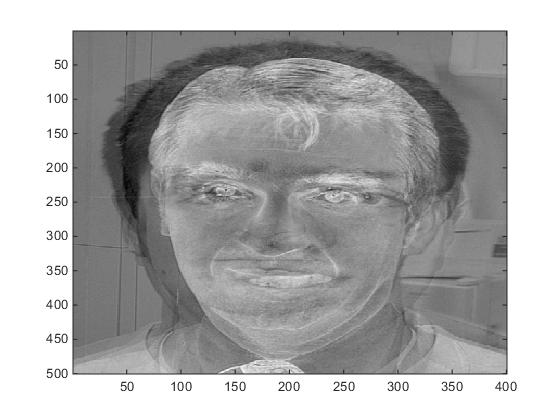
\includegraphics[width=0.95\textwidth]{img/fr/eigenface1.jpg}
  \caption{}
  % \label{fig:sub1}
\end{subfigure}%
\begin{subfigure}{.24\textwidth}
  \centering
  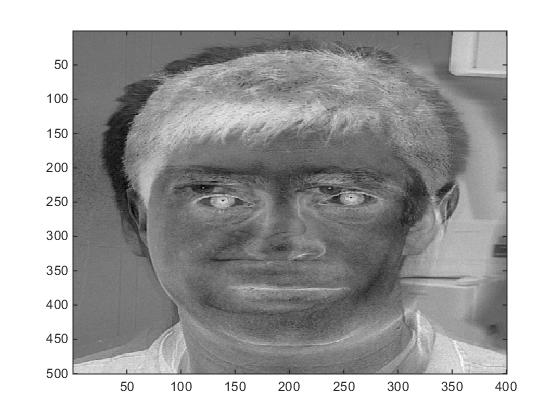
\includegraphics[width=0.95\textwidth]{img/fr/eigenface2.jpg}
  \caption{}
  % \label{fig:sub1}
\end{subfigure}%
\begin{subfigure}{.24\textwidth}
  \centering
  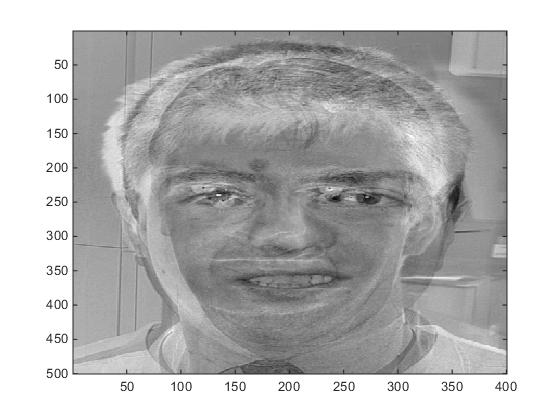
\includegraphics[width=0.95\textwidth]{img/fr/eigenface3.jpg}
  \caption{}
  % \label{fig:sub1}
\end{subfigure}%
\begin{subfigure}{.24\textwidth}
  \centering
  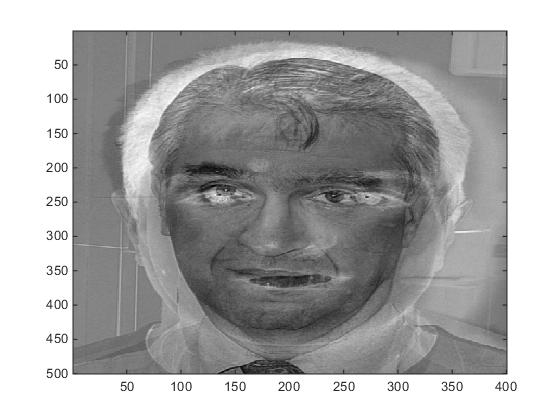
\includegraphics[width=0.95\textwidth]{img/fr/eigenface4.jpg}
  \caption{}
  % \label{fig:sub1}
\end{subfigure}%

\caption{Example of some eigenfaces from our database.}
\label{fig:eigenface}
\end{figure}
